\begin{frame}{Überblick Vortrag}
\small
\begin{itemize}\setlength{\itemsep}{3mm}
  \item \textbf{Einführung und Ziele}
  \item \textbf{1. Rahmeninfos:} Pinecil, Temperatur, Spitzenpflege, Spitzenaktivator
  \item \textbf{2. Sicherheit:} Hitze, Arbeitsplatz, Dämpfe, Schutz, Verhalten, Erste Hilfe
  \item \textbf{3. Kurze Geschichte:} Antike, Elektronik
\end{itemize}
\end{frame}

\begin{frame}{Überblick Vortrag}
\begin{itemize}\setlength{\itemsep}{3mm}
  \item \textbf{4. Wozu und Arten:} Was ist Löten, Anwendungen, Lötarten, THT, SMD
  \item \textbf{5. Werkzeuge und Material:} Lötstation, Spitzen, Lötzinn, Flussmittel, Entlöten, Helfer
  \item \textbf{6. Techniken und Methoden:} Gute Lötstelle, Vorbereitung, Wärmeführung, Zinn zuführen, Absetzen, Nacharbeit, Temperatur und Zeit
\end{itemize}
\end{frame}

\begin{frame}{Überblick Vortrag}
\begin{itemize}\setlength{\itemsep}{3mm}
  \item \textbf{7. Häufige Fehler und Lösungen:} Kalte Lötstelle, zu viel, zu wenig, Brücke, Überhitzung, Bauteil schief
  \item \textbf{8. Kontrolle und Praxis:} Inspektion, elektrische Prüfung, Ablauf Praxis, Merkhilfe
  \item \textbf{9. Projekte nach Erfahrungsstufe:} Stufen 1 bis 5, Sicherheit, Material, Vorstellung
  \item \textbf{Q \& A und Abschluss}
\end{itemize}
\normalsize
\end{frame}


\begin{frame}{Einführung ins Löten}
    \begin{itemize}\setlength{\itemsep}{3mm}
        \item \begin{center}\textbf{Ziel heute}: sicher löten lernen\end{center}
        \item \begin{center}\textbf{Überblick}: Vortrag mit Sicherheit, Grundlagen und dann Praxis\end{center}
    \end{itemize}
\end{frame}


\begin{frame}{Was nimmst du mit ?}
\begin{itemize}\setlength{\itemsep}{3mm}
  \item - Sicherer Umgang mit dem Lötkolben
  \item - Kenntnis der Werkzeuge und Materialien
  \item - Gute Lötstellen erkennen
  \item - Fehler vermeiden und beheben
\end{itemize}
\end{frame}






\begin{frame}{Temperaturrichtlinien}
\begin{columns}[T]
    \begin{column}{0.58\textwidth}
        \small
        \begin{itemize}\setlength{\itemsep}{3mm}
            \item THT bleifrei meist 340 bis 370 Grad
            \item Feine Pads 320 bis 350 Grad
            \item Masseflächen kurz etwas höher mit Boost
        \end{itemize}
        \normalsize
    \end{column}
    \begin{column}{0.42\textwidth}
        \centering
        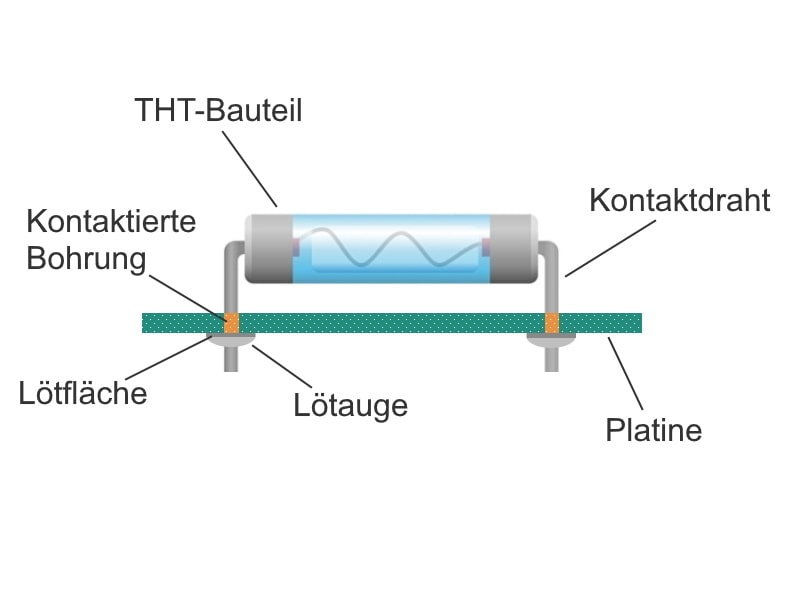
\includegraphics[width=\linewidth,keepaspectratio]{2.0.0.0_content/assets/bilder/tht_löten.jpg}
    \end{column}
\end{columns}
\end{frame}

\begin{frame}{Spitzenpflege}
\begin{itemize}\setlength{\itemsep}{3mm}
    \item - Reinigung mit Messingwolle
    \item - Spitze dünn verzinnen
    \item - Feuchter Schwamm optional (haben wir aber nicht)
\end{itemize}
\end{frame}

\begin{frame}{Spitzenaktivator}
\begin{itemize}\setlength{\itemsep}{3mm}
    \item - Aktivator für stumpfe Spitzen
    \item - Sparsam einsetzen
    \item - Danach sofort neu verzinnen
\end{itemize}
\end{frame}

% Block 1: Sicherheit
\begin{frame}{Hitze verstehen}
\begin{itemize}\setlength{\itemsep}{3mm}
    \item - Pinecil kann sehr heiß werden bis zu 450 °C
    \item - Spitze nie berühren
    \item - Nur in der Halterung/Matte ablegen
\end{itemize}
\end{frame}

\begin{frame}{Arbeitsplatz}
\begin{columns}[T]
    \begin{column}{0.58\textwidth}
        \small
        \begin{itemize}\setlength{\itemsep}{3mm}
            \item Aufgeräumt und gut beleuchtet
            \item Wärmeresistente Unterlage
            \item Kabel sicher führen
        \end{itemize}
        \normalsize
    \end{column}
    \begin{column}{0.42\textwidth}
        \centering
        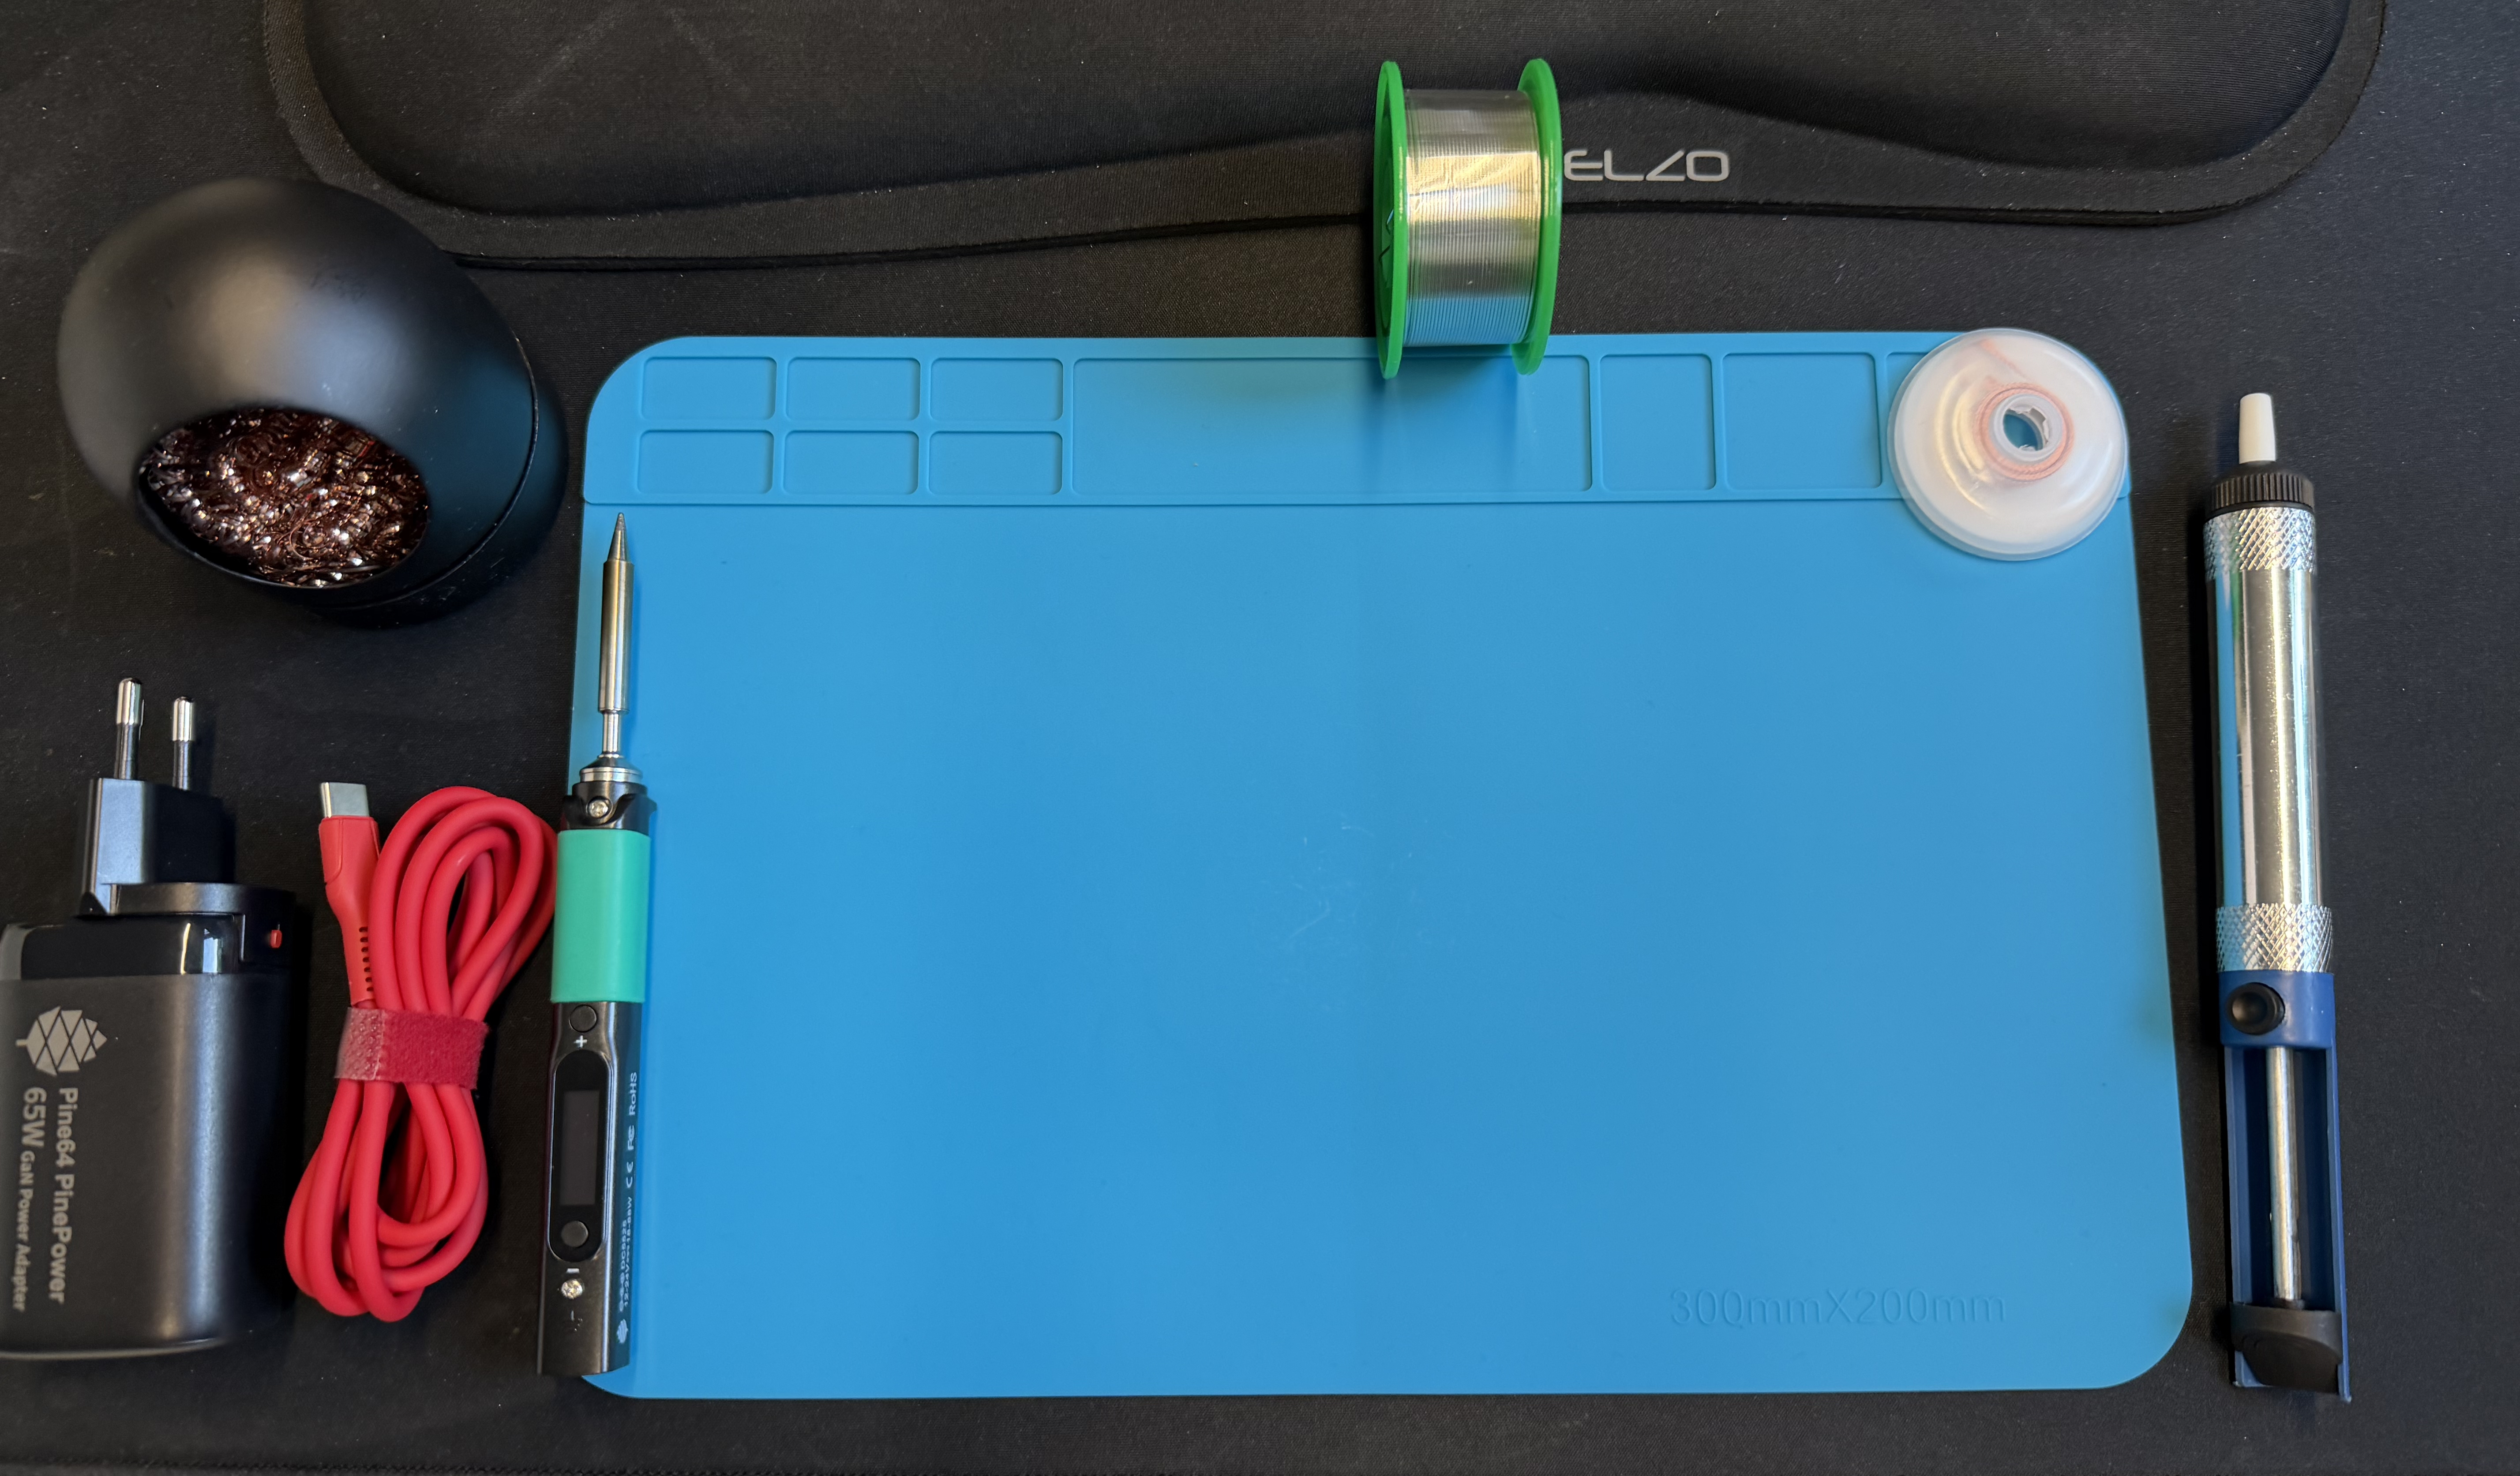
\includegraphics[width=\linewidth,keepaspectratio]{2.0.0.0_content/assets/bilder/setup.jpg}
    \end{column}
\end{columns}
\end{frame}

\begin{frame}{Dämpfe und Luft}
\begin{itemize}\setlength{\itemsep}{3mm}
    \item - Gut lüften
    \item - Rauch nicht einatmen
    \item - Absaugung bei Bedarf
\end{itemize}
\end{frame}

\begin{frame}{Schutz und Verhalten}
\begin{itemize}\setlength{\itemsep}{3mm}
    \item - Schutzbrille bei Drahtarbeiten
    \item - Keine Getränke an der Lötstelle
    \item - Nicht mit Kolben herumlaufen
\end{itemize}
\end{frame}

% Block 2: Kurze Geschichte
\begin{frame}{Von der Antike bis heute}
\begin{itemize}\setlength{\itemsep}{3mm}
    \item - Ursprung in Schmuck und Metall
    \item - Zusatzmetall verbindet Basismetalle
    \item - Prinzip unverändert
\end{itemize}
\end{frame}

\begin{frame}{Elektronik}
\begin{itemize}\setlength{\itemsep}{3mm}
    \item - Standard in der Fertigung
    \item - Handlöten wichtig für Prototypen und Repair
\end{itemize}
\end{frame}

% Block 3: Wozu und welche Arten
\begin{frame}{Was ist Löten}
\begin{itemize}\setlength{\itemsep}{3mm}
    \item - Lot schmilzt, Bauteile bleiben fest
    \item - Verbindung ist elektrisch leitend und mechanisch stabil
\end{itemize}
\end{frame}

\begin{frame}{Typische Anwendungen}
\begin{itemize}\setlength{\itemsep}{3mm}
    \item - Platinenaufbau
    \item - Reparatur und Modding
    \item - Maker Projekte wie LED, Sensoren, Mikrocontroller
\end{itemize}
\end{frame}

\begin{frame}{Lötarten}
\begin{columns}[T]
    \begin{column}{0.58\textwidth}
        \small
        \begin{itemize}\setlength{\itemsep}{3mm}
            \item \textbf{Weichlöten} in der Elektronik
            \item \textbf{Hartlöten} im Metallbau
        \end{itemize}
        \normalsize
    \end{column}
    \begin{column}{0.42\textwidth}
        \centering
        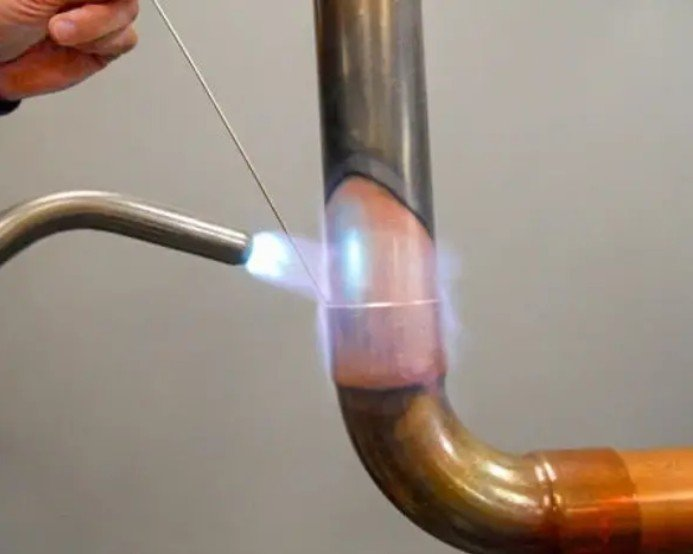
\includegraphics[width=\linewidth,keepaspectratio]{2.0.0.0_content/assets/bilder/hartlöten.jpg}
    \end{column}
\end{columns}
\end{frame}

\begin{frame}{THT und SMD}
\begin{itemize}\setlength{\itemsep}{3mm}
    \item - THT: Beinchen durch Löcher
    \item - SMD: Bauteile auf Pads
    \item - Heute Fokus auf THT
\end{itemize}
\end{frame}

% Block 4: Werkzeuge und Material
\begin{frame}{Lötstation im Detail}
\begin{itemize}\setlength{\itemsep}{3mm}
    \item - Temperaturregelung und Sleep
    \item - Halterung und Ablage
    \item - Auto Standby zum Schutz
\end{itemize}
\end{frame}

\begin{frame}{Spitzenformen}
\begin{itemize}\setlength{\itemsep}{3mm}
    \item - Meißel für Pads und Wärmeübertrag
    \item - Konisch für feine Punkte
    \item - Spitze passend zur Aufgabe wählen
\end{itemize}
\end{frame}

\begin{frame}{Lötzinn}
\begin{itemize}\setlength{\itemsep}{3mm}
    \item - Flussmittelkern integriert
    \item - 0.5 bis 1.0 mm üblich
    \item - Bleifrei bevorzugt
\end{itemize}
\end{frame}

\begin{frame}{Entlöten}
\begin{itemize}\setlength{\itemsep}{3mm}
    \item - Pumpe für viel Zinn
    \item - Litze für präzise Aufnahme
    \item - Geduld statt Kraft
\end{itemize}
\end{frame}

\begin{frame}{Nützliche Helfer}
\begin{itemize}\setlength{\itemsep}{3mm}
    \item - Dritter Arm und Pinzette
    \item - Seitenschneider
    \item - Messingwolle oder Schwamm
\end{itemize}
\end{frame}

% Block 5: Techniken und Methoden
\begin{frame}{Gute Lötstelle}
\begin{itemize}\setlength{\itemsep}{3mm}
    \item - Leicht glänzend, glatte Oberfläche
    \item - Kegelförmig, Pin gut umflossen
    \item - Keine Brücken, mechanisch fest
\end{itemize}
\end{frame}

\begin{frame}{Vorbereitung}
\begin{itemize}\setlength{\itemsep}{3mm}
    \item - Bauteil einsetzen, Beinchen leicht spreizen
    \item - Spitze sauber, kurz benetzen
    \item - Kontaktflächen sauber und fixiert
\end{itemize}
\end{frame}

\begin{frame}{Wärmeführung}
\begin{itemize}\setlength{\itemsep}{3mm}
    \item - Spitze an Pad und Pin
    \item - Erst erwärmen, dann Zinn zuführen
\end{itemize}
\end{frame}

\begin{frame}{Zinn zuführen}
\begin{itemize}\setlength{\itemsep}{3mm}
    \item - Zinn an die Stelle, nicht an die Spitze
    \item - Kapillarwirkung nutzen
    \item - Weniger ist oft besser
\end{itemize}
\end{frame}

\begin{frame}{Absetzen und Prüfen}
\begin{itemize}\setlength{\itemsep}{3mm}
    \item - Zinn weg, dann Spitze weg
    \item - Kurz ruhen lassen
    \item - Sichtprüfung
\end{itemize}
\end{frame}

\begin{frame}{Nacharbeit}
\begin{itemize}\setlength{\itemsep}{3mm}
    \item - Beinchen kürzen
    \item - Keine Bewegung beim Abkühlen
    \item - Bei Zweifel neu aufbauen
\end{itemize}
\end{frame}

\begin{frame}{Temperatur und Zeit}
\begin{itemize}\setlength{\itemsep}{3mm}
    \item - Nicht zu kalt, nicht zu heiß
    \item - Kurz, sauber, kontrolliert
    \item - Boost nur wenige Sekunden
\end{itemize}
\end{frame}

% Block 6: Häufige Fehler und Lösungen
\begin{frame}{Kalte Lötstelle}
\begin{itemize}\setlength{\itemsep}{3mm}
    \item - Matt, körnig, wackelt
    \item - Lösung: erneut erwärmen, wenig Zinn zugeben
\end{itemize}
\end{frame}

\begin{frame}{Zu viel Zinn}
\begin{itemize}\setlength{\itemsep}{3mm}
    \item - Kugelbildung, Risiko von Brücken
    \item - Lösung: erwärmen, Pumpe oder Litze nutzen
\end{itemize}
\end{frame}

\begin{frame}{Zu wenig Zinn}
\begin{itemize}\setlength{\itemsep}{3mm}
    \item - Pad kaum benetzt, schwache Verbindung
    \item - Lösung: nachführen und erneut erwärmen
\end{itemize}
\end{frame}

\begin{frame}{Lötbrücke}
\begin{itemize}\setlength{\itemsep}{3mm}
    \item - Kurzschluss zwischen Pads
    \item - Lösung: Litze nutzen, sauber abheben
\end{itemize}
\end{frame}

\begin{frame}{Überhitzung}
\begin{itemize}\setlength{\itemsep}{3mm}
    \item - Pad verfärbt, Bauteil leidet
    \item - Lösung: kürzere Erwärmung, Pausen
\end{itemize}
\end{frame}

\begin{frame}{Bauteil schief}
\begin{itemize}\setlength{\itemsep}{3mm}
    \item - Optisch und mechanisch schlecht
    \item - Lösung: verflüssigen, neu ausrichten
\end{itemize}
\end{frame}

% Block 7: Kontrolle und Praxis
\begin{frame}{Inspektion}
\begin{itemize}\setlength{\itemsep}{3mm}
    \item - Lupe oder Kamera
    \item - Gleichmäßige Form
    \item - Keine Risse oder Löcher
\end{itemize}
\end{frame}

\begin{frame}{Elektrische Prüfung}
\begin{itemize}\setlength{\itemsep}{3mm}
    \item - Durchgang testen
    \item - Kurzschlusscheck
\end{itemize}
\end{frame}

\begin{frame}{Ablauf Praxis}
\begin{itemize}\setlength{\itemsep}{3mm}
    \item - Demo
    \item - Testplatine
    \item - Projekt löten und mitnehmen
\end{itemize}
\end{frame}

\begin{frame}{Merkhilfe}
\begin{itemize}\setlength{\itemsep}{3mm}
    \item - Wärme in die Verbindung
    \item - Zinn an das Werkstück
    \item - Ruhe beim Abkühlen
\end{itemize}
\end{frame}

% Block 8: Projekte nach Erfahrungsstufe
\begin{frame}{Überblick Projekte}
\begin{itemize}\setlength{\itemsep}{3mm}
  \item Fünf Stufen nach Erfahrung
  \item Projekte zum Mitnehmen
  \item Zeit 10 bis 40 Minuten
\end{itemize}
\end{frame}

% Taschenrechner
\begin{frame}{Taschenrechner Projekt}
\begin{columns}[T]
  \begin{column}{0.58\textwidth}
    \small
    \begin{itemize}\setlength{\itemsep}{3mm}
      \item THT Taschenrechner Bausatz
      \item Widerstände, IC, Taster und Quarz
      \item Lernziel: Reihenfolge und saubere Wärmeführung
    \end{itemize}
    \normalsize
  \end{column}
  \begin{column}{0.42\textwidth}
    \centering
    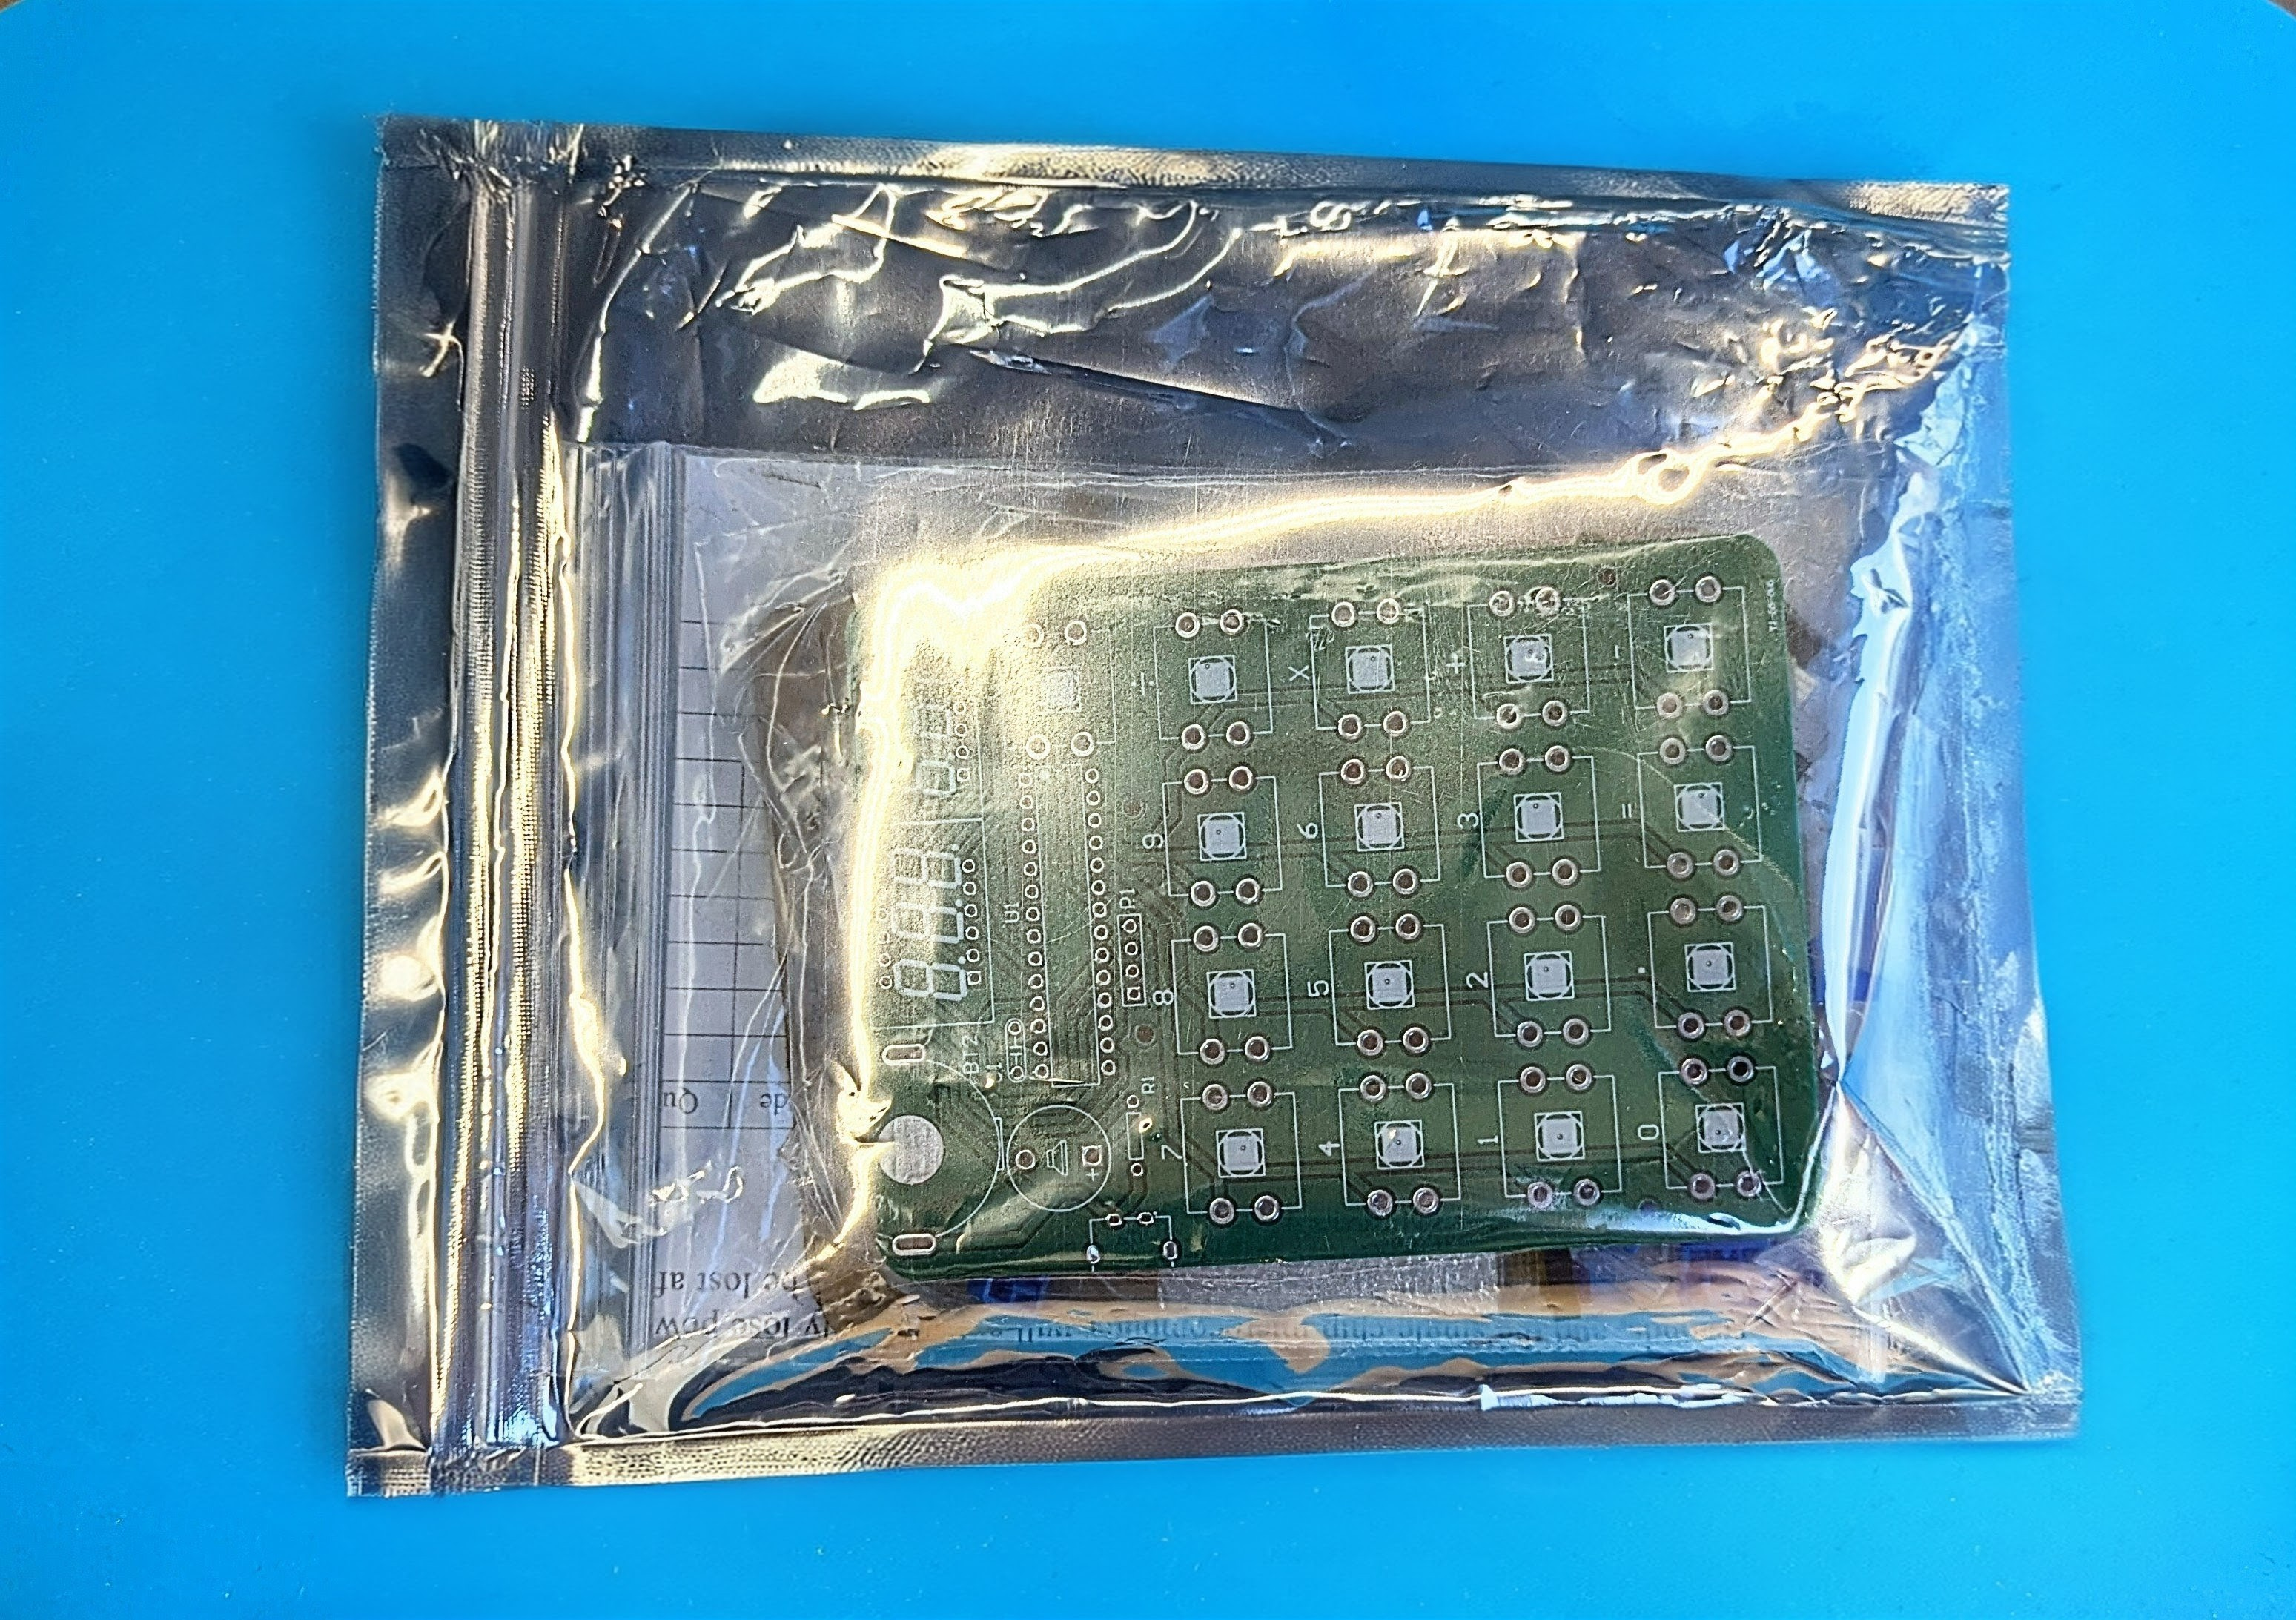
\includegraphics[width=\linewidth,keepaspectratio]{2.0.0.0_content/assets/bilder/projekt_calc.jpg}
  \end{column}
\end{columns}
\end{frame}

\begin{frame}{Taschenrechner fertig}
\begin{columns}[T]
  \begin{column}{0.58\textwidth}
    \small
    \begin{itemize}\setlength{\itemsep}{3mm}
      \item Funktion geprüft und einsatzbereit
      \item Alle Lötstellen kontrolliert
      \item Mitnahme nach kurzem Test möglich
    \end{itemize}
    \normalsize
  \end{column}
  \begin{column}{0.42\textwidth}
    \centering
    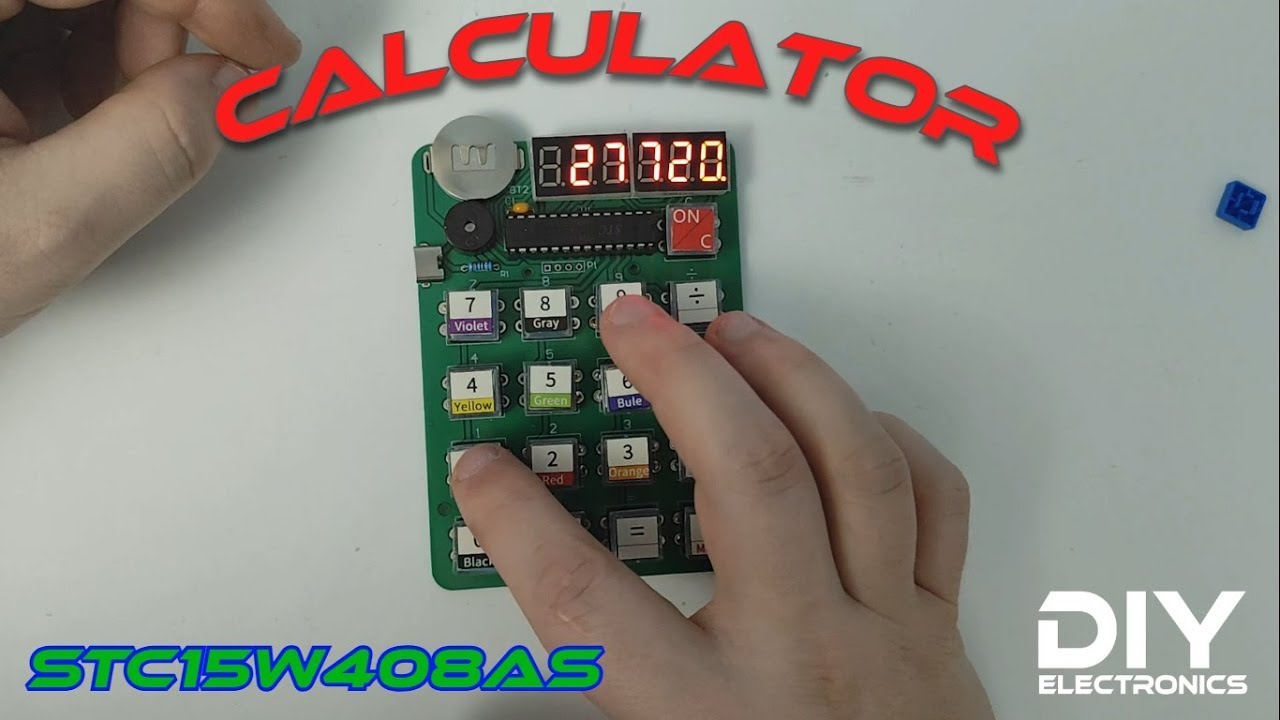
\includegraphics[width=\linewidth,keepaspectratio]{2.0.0.0_content/assets/bilder/projekt_calc_fertig.jpg}
  \end{column}
\end{columns}
\end{frame}

% Uhr
\begin{frame}{Uhr Projekt}
\begin{columns}[T]
  \begin{column}{0.58\textwidth}
    \small
    \begin{itemize}\setlength{\itemsep}{3mm}
      \item Digitale Uhr als Bausatz
      \item Display und mehrere THT Bauteile
      \item Lernziel: Serienlöten und Bauteilorientierung
    \end{itemize}
    \normalsize
  \end{column}
  \begin{column}{0.42\textwidth}
    \centering
    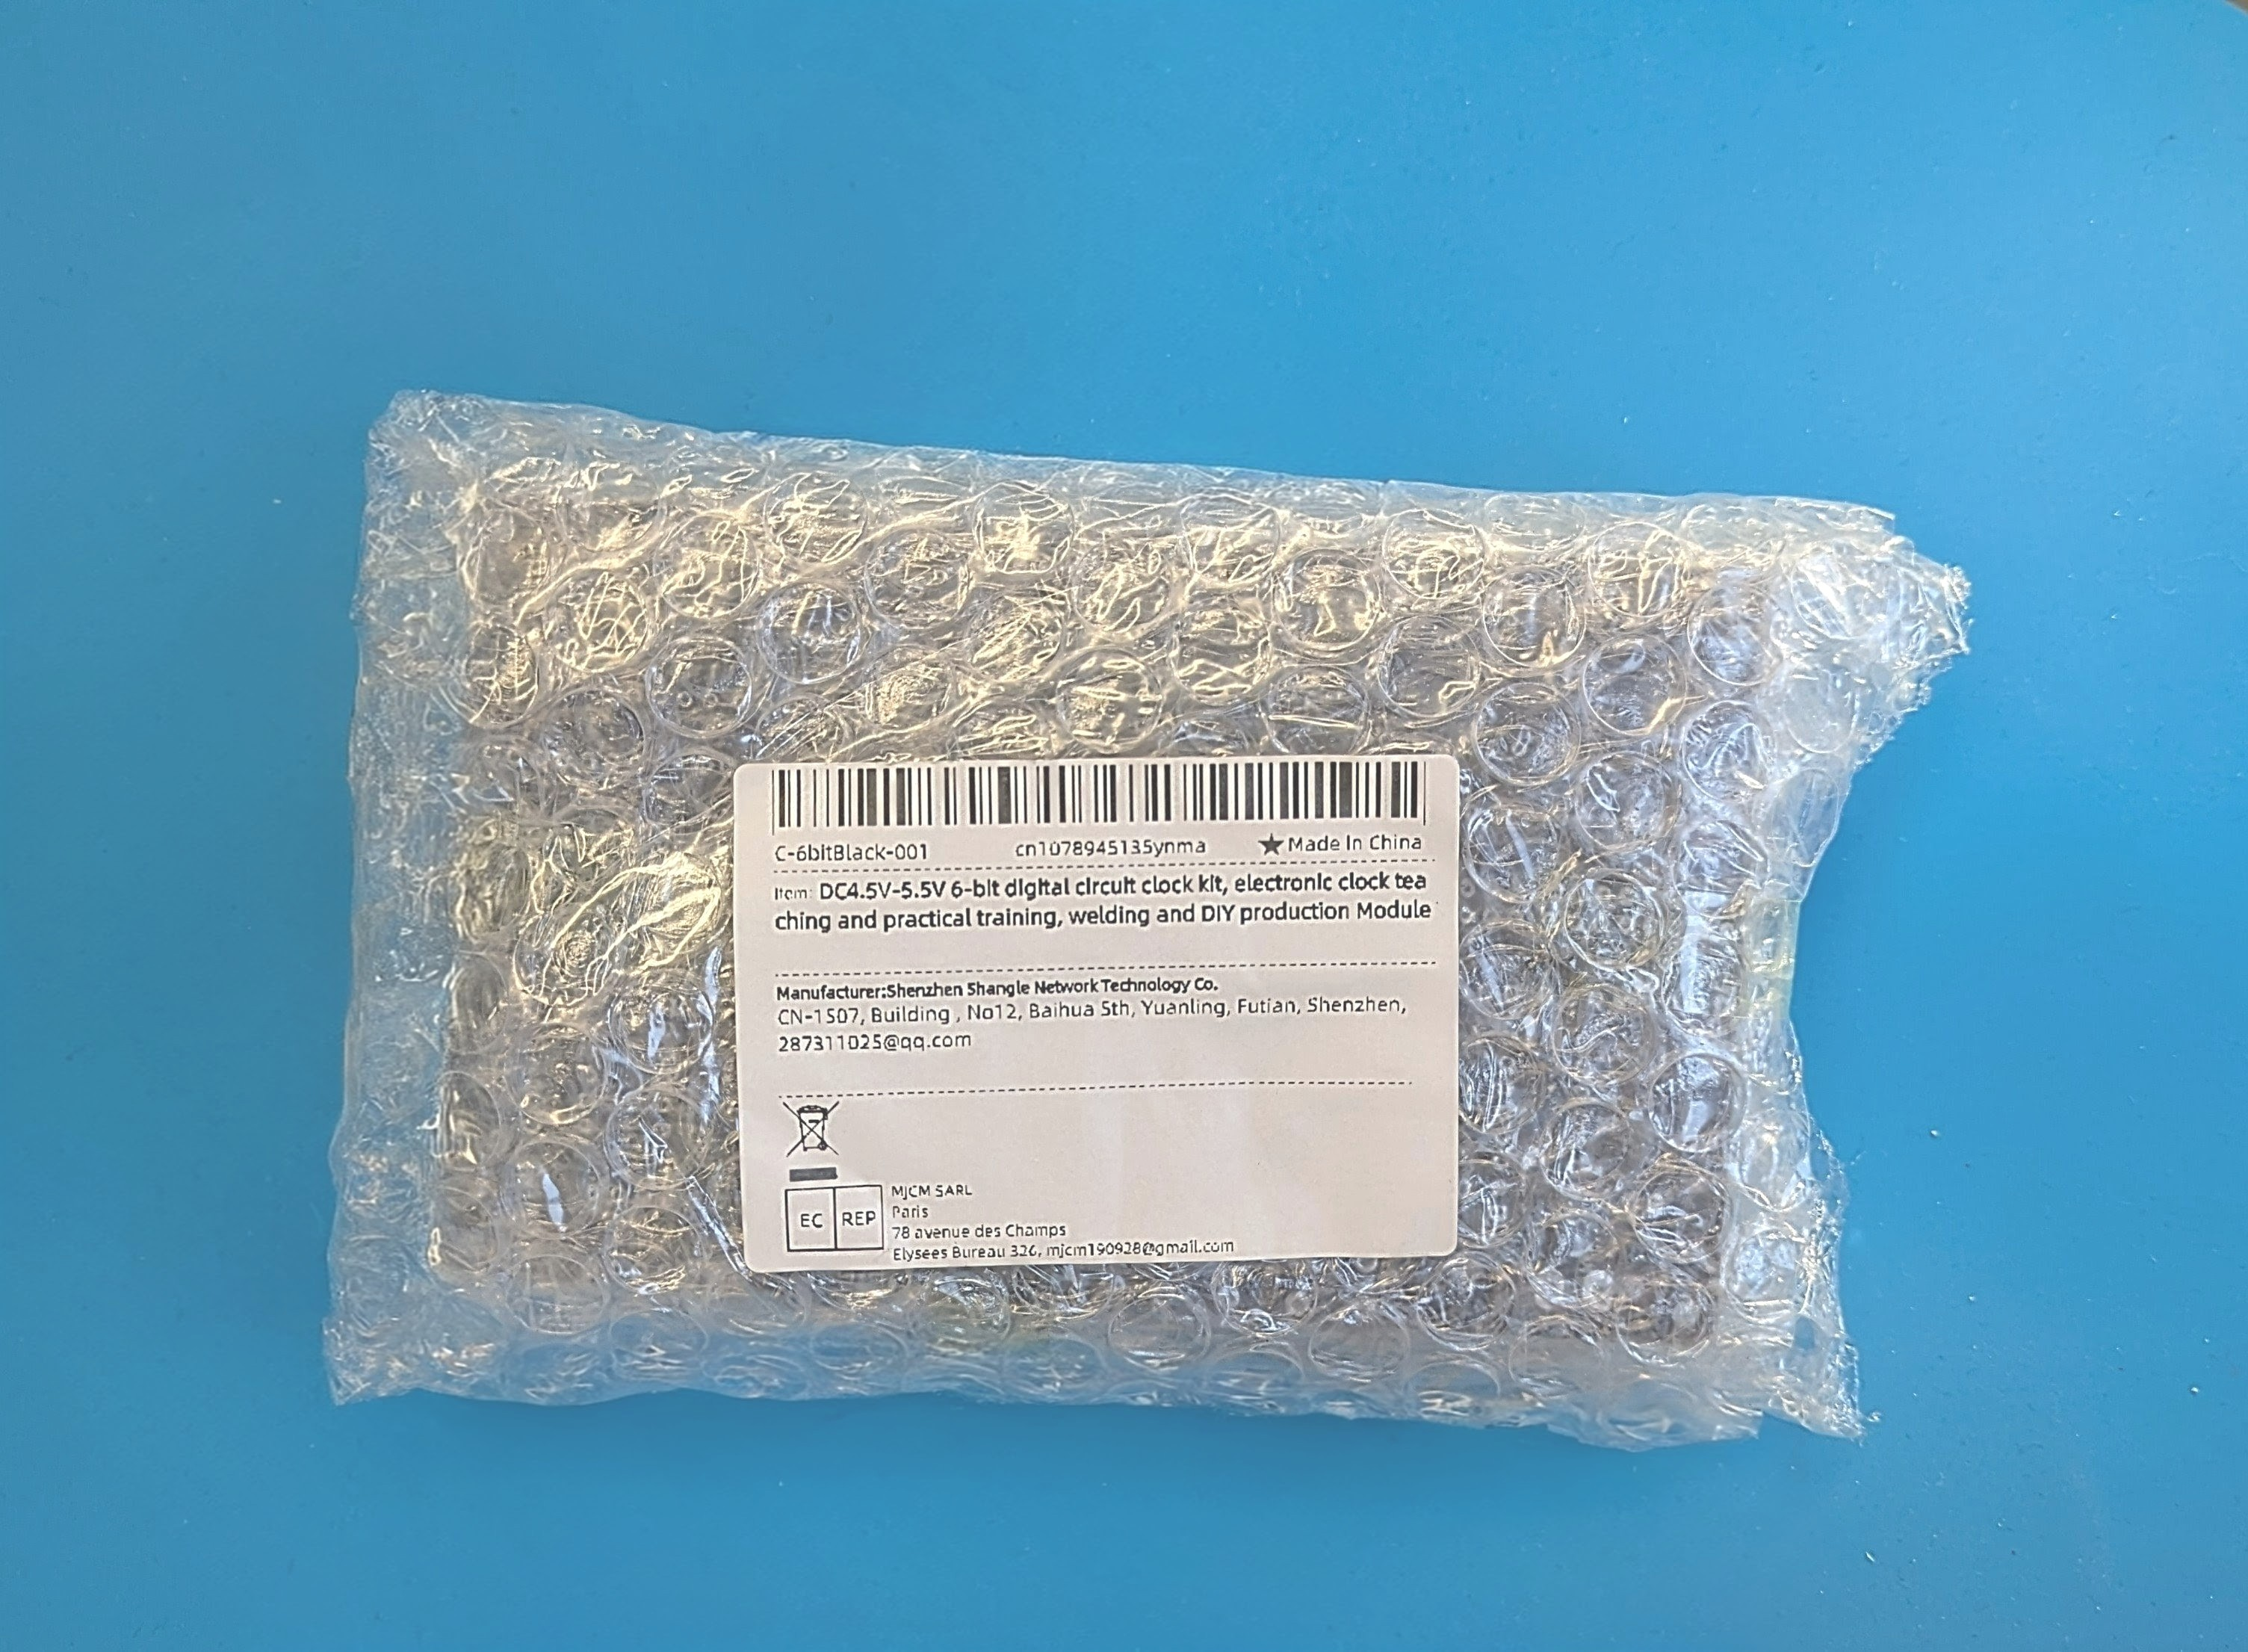
\includegraphics[width=\linewidth,keepaspectratio]{2.0.0.0_content/assets/bilder/projekt_clock.jpg}
  \end{column}
\end{columns}
\end{frame}

\begin{frame}{Uhr fertig}
\begin{columns}[T]
  \begin{column}{0.58\textwidth}
    \small
    \begin{itemize}\setlength{\itemsep}{3mm}
      \item Uhr läuft stabil
      \item Saubere Lötstellen ohne Brücken
      \item Optionales Gehäuse möglich
    \end{itemize}
    \normalsize
  \end{column}
  \begin{column}{0.42\textwidth}
    \centering
    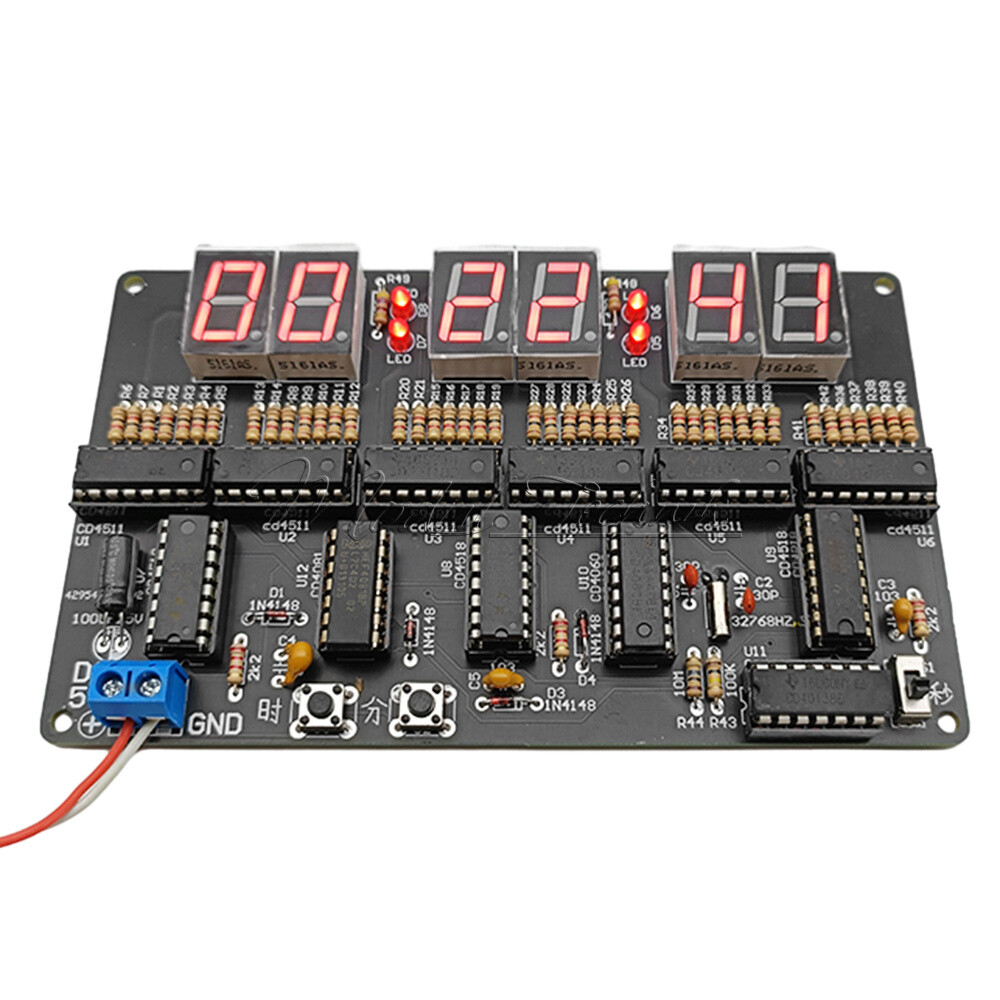
\includegraphics[width=\linewidth,keepaspectratio]{2.0.0.0_content/assets/bilder/projekt_clock_fertig.jpg}
  \end{column}
\end{columns}
\end{frame}

% ESP Wetter Uhr
\begin{frame}{ESP Wetter Uhr Projekt}
\begin{columns}[T]
  \begin{column}{0.58\textwidth}
    \small
    \begin{itemize}\setlength{\itemsep}{3mm}
      \item ESP Mikrocontroller mit Sensor
      \item Anzeige von Zeit und Wetter
      \item Lernziel: Stiftleisten, Kabel und Temperaturdisziplin
    \end{itemize}
    \normalsize
  \end{column}
  \begin{column}{0.42\textwidth}
    \centering
    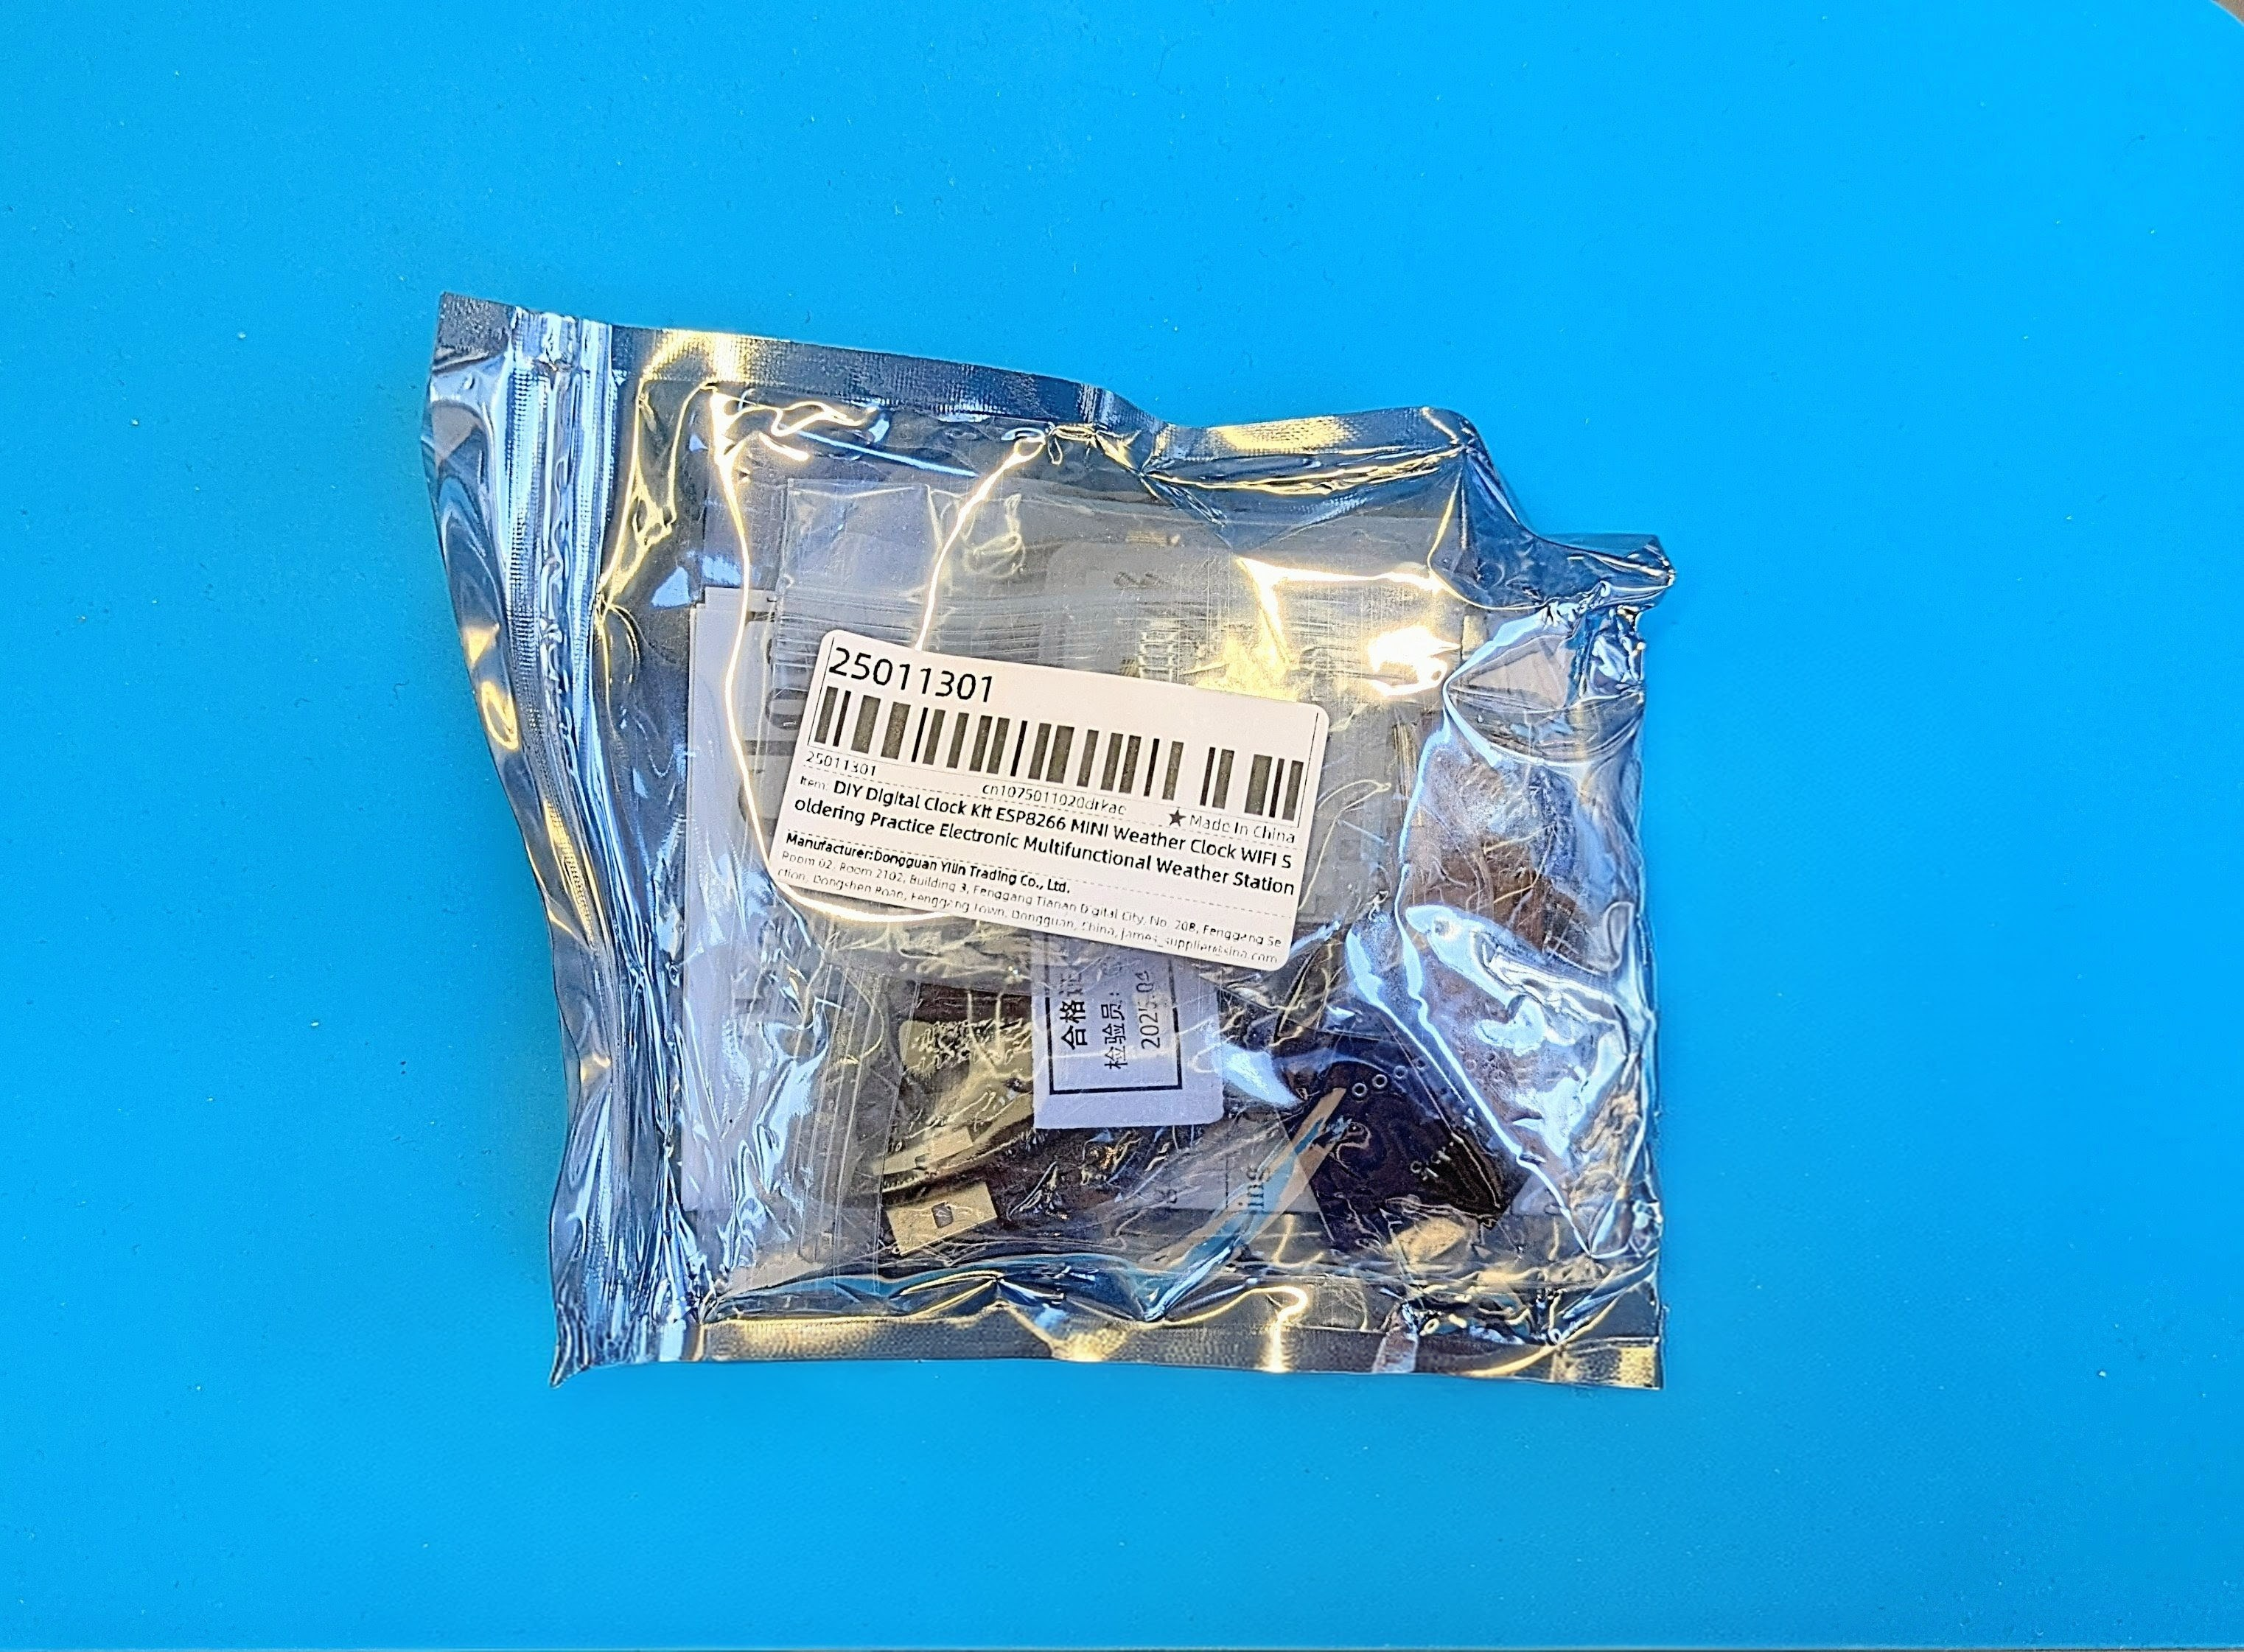
\includegraphics[width=\linewidth,keepaspectratio]{2.0.0.0_content/assets/bilder/projekt_esp_wetter_uhr_1.jpg}
  \end{column}
\end{columns}
\end{frame}

\begin{frame}{ESP Wetter Uhr fertig}
\begin{columns}[T]
  \begin{column}{0.58\textwidth}
    \small
    \begin{itemize}\setlength{\itemsep}{3mm}
      \item Anzeige getestet und lesbar
      \item Stromversorgung geprüft
      \item Bereit zum Mitnehmen
    \end{itemize}
    \normalsize
  \end{column}
  \begin{column}{0.42\textwidth}
    \centering
    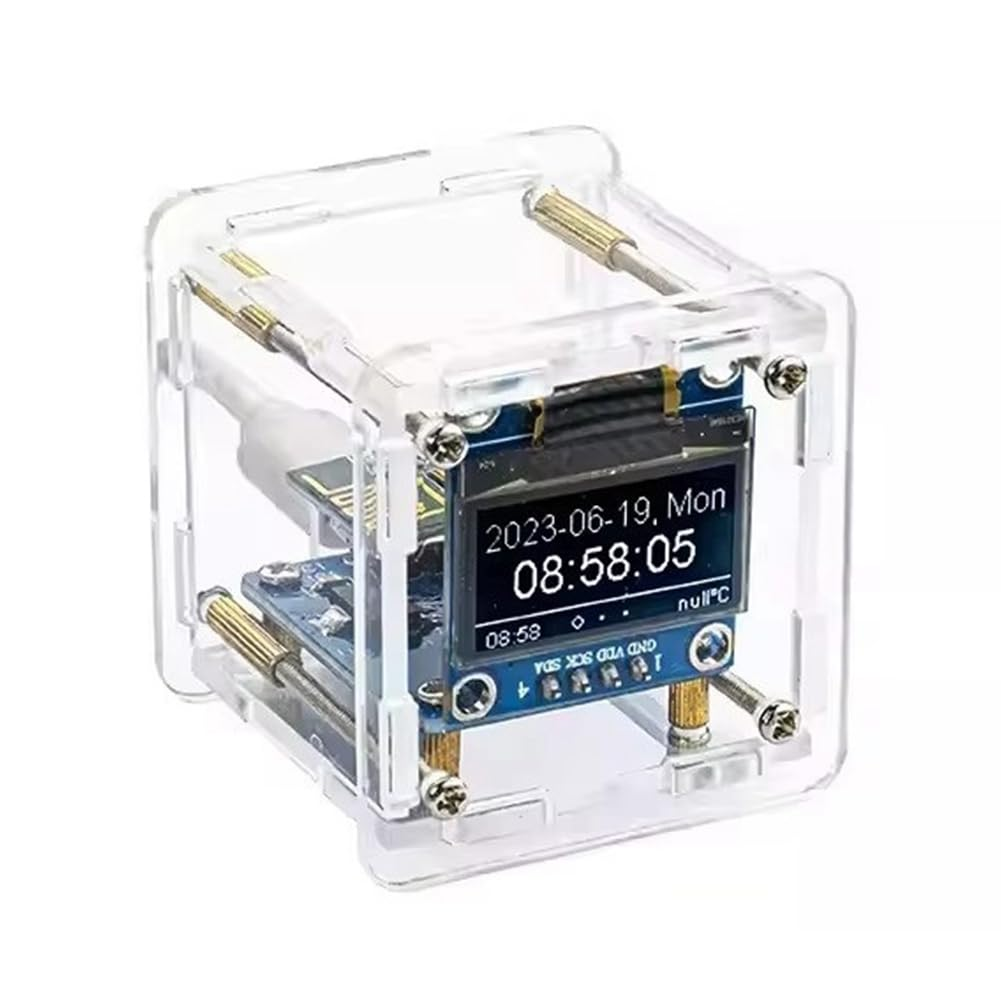
\includegraphics[width=\linewidth,keepaspectratio]{2.0.0.0_content/assets/bilder/projekt_esp_wetter_clock_fertig.jpg}
  \end{column}
\end{columns}
\end{frame}

% GB Projekt
\begin{frame}{GB Projekt}
\begin{columns}[T]
  \begin{column}{0.58\textwidth}
    \small
    \begin{itemize}\setlength{\itemsep}{3mm}
      \item Mehrteiliger Bausatz mit LEDs und Tastern
      \item Saubere Lötstellen auf engem Raum
      \item Lernziel: ruhige Hand und kurze Lötzeiten
    \end{itemize}
    \normalsize
  \end{column}
  \begin{column}{0.42\textwidth}
    \centering
    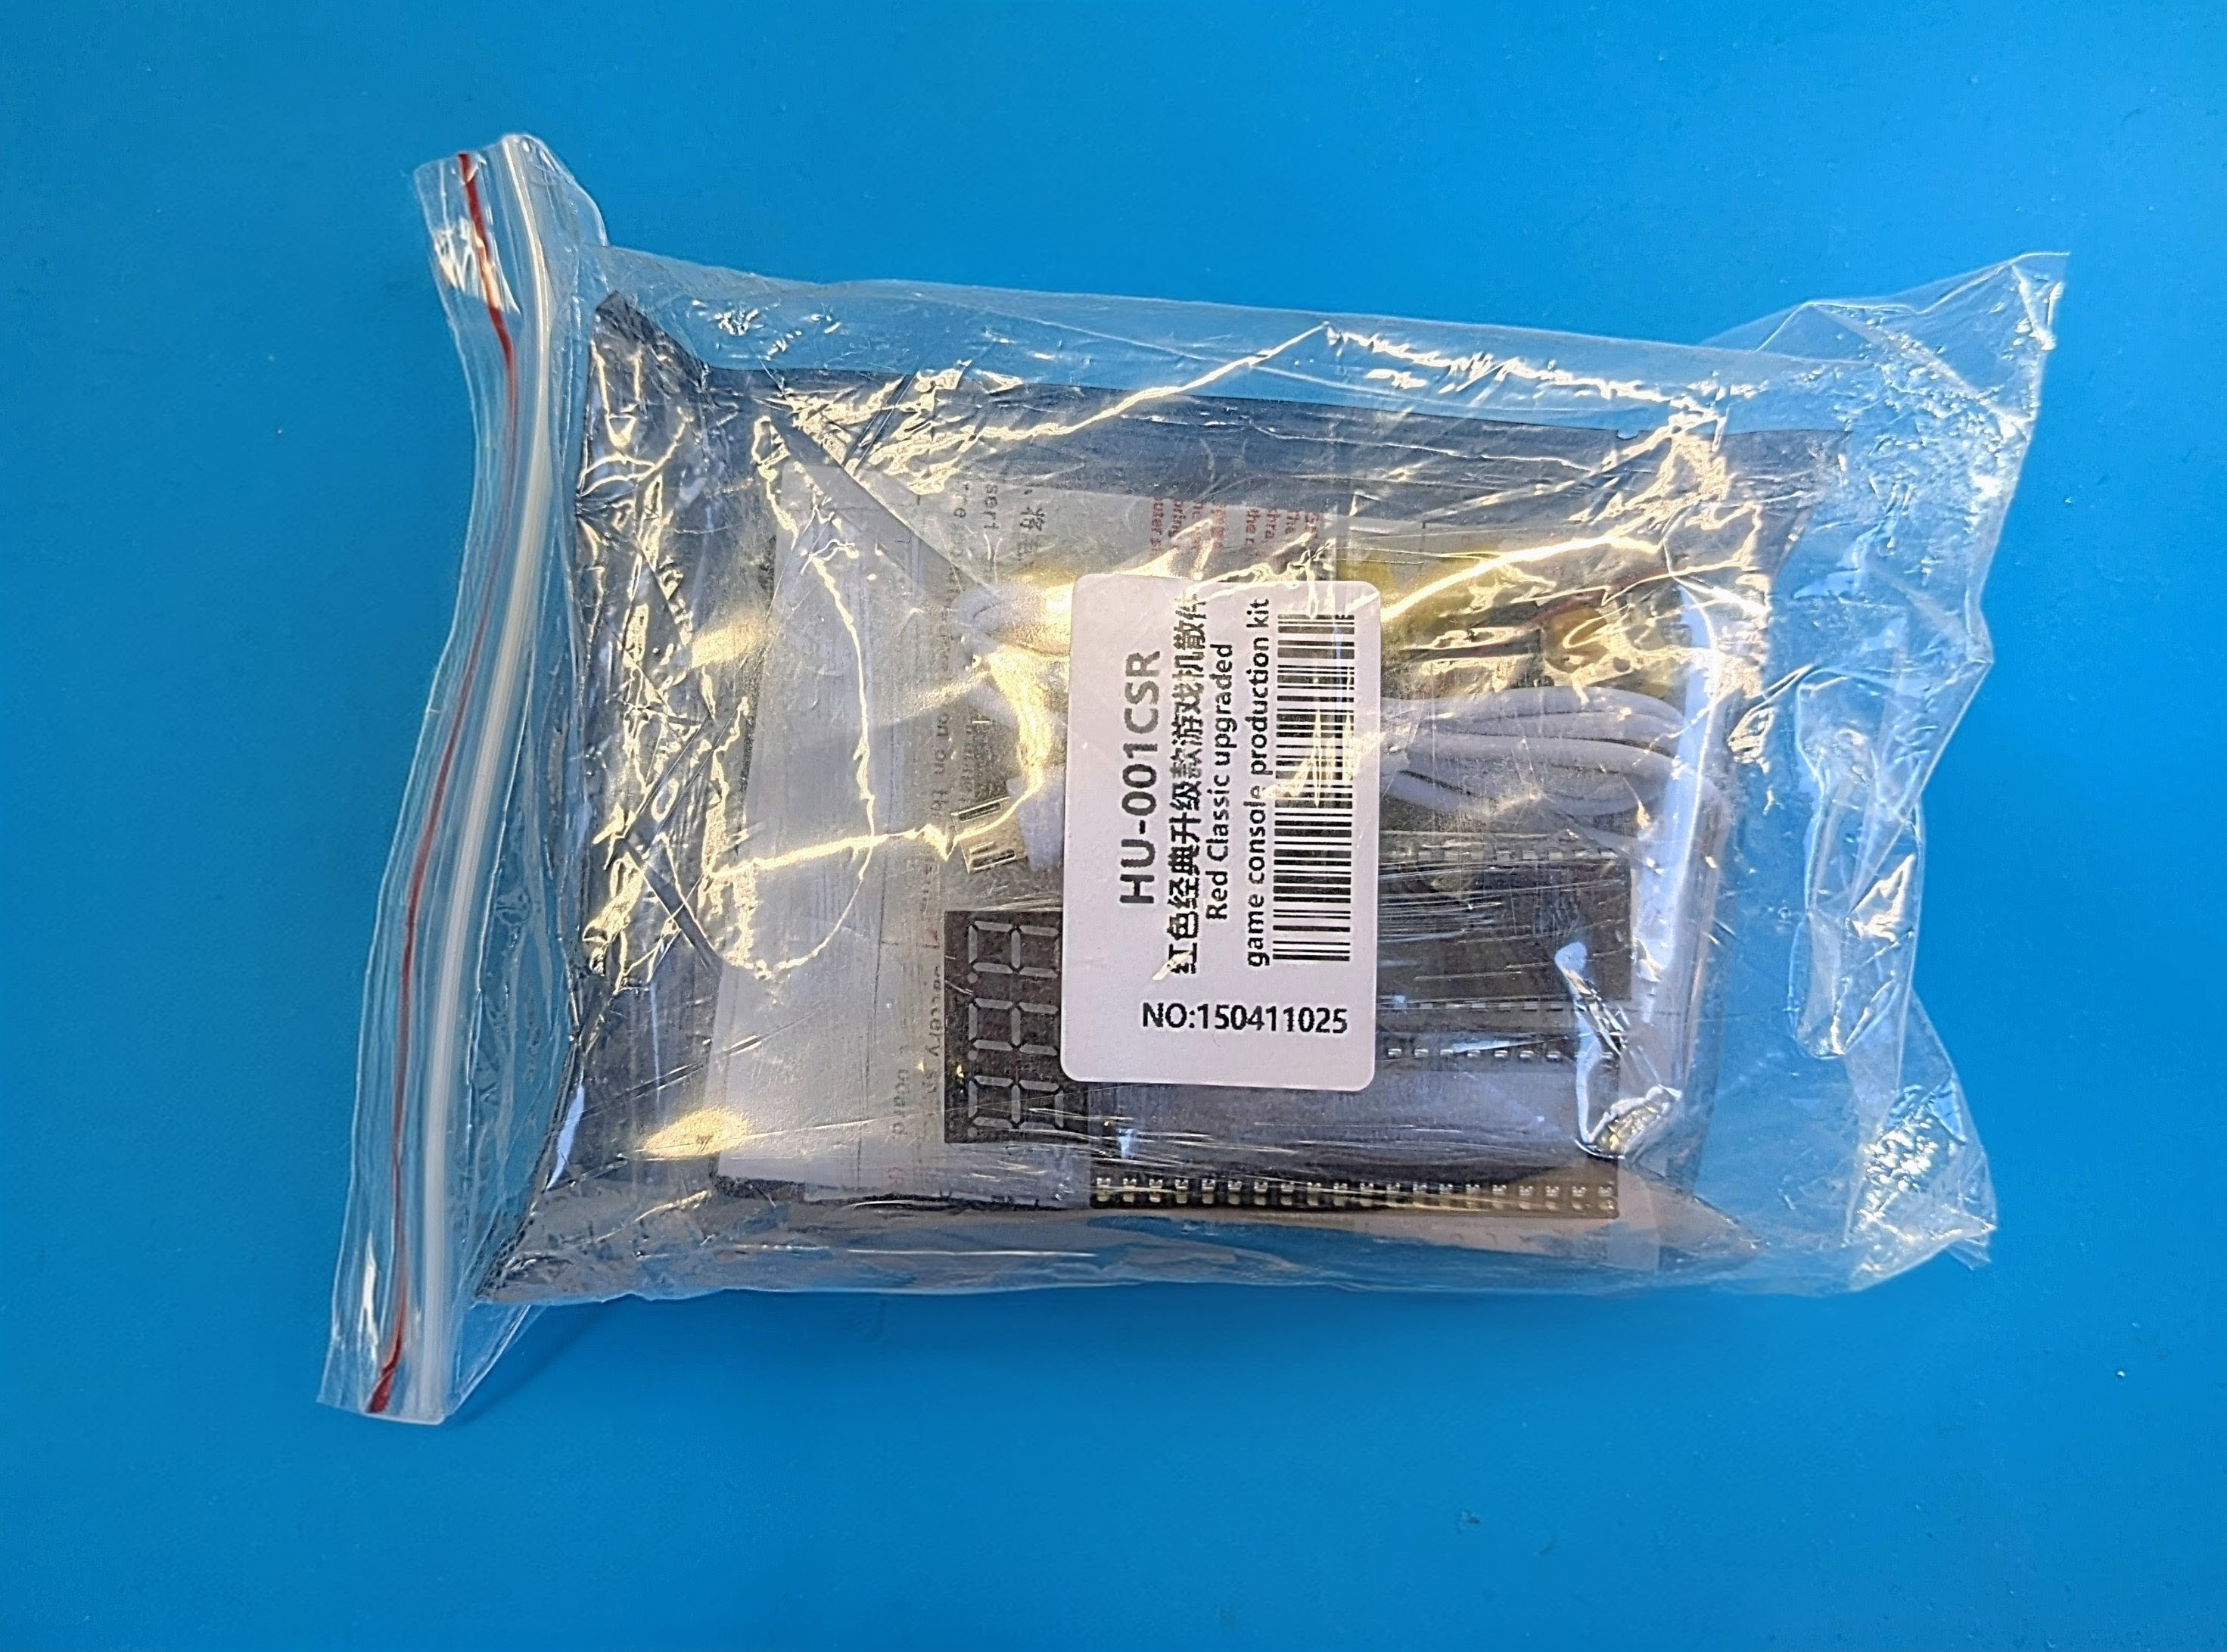
\includegraphics[width=\linewidth,keepaspectratio]{2.0.0.0_content/assets/bilder/projekt_gb_1.jpg}
  \end{column}
\end{columns}
\end{frame}

\begin{frame}{GB fertig}
\begin{columns}[T]
  \begin{column}{0.58\textwidth}
    \small
    \begin{itemize}\setlength{\itemsep}{3mm}
      \item Funktion getestet
      \item Mechanisch stabil
      \item Mitnahme möglich
    \end{itemize}
    \normalsize
  \end{column}
  \begin{column}{0.42\textwidth}
    \centering
    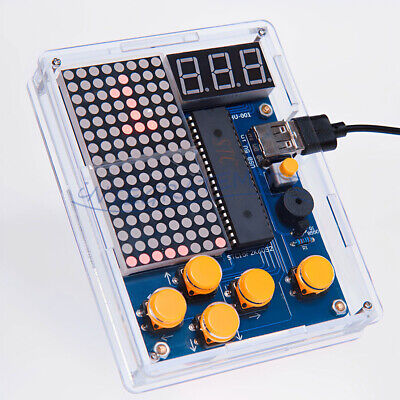
\includegraphics[width=\linewidth,keepaspectratio]{2.0.0.0_content/assets/bilder/projekt_gb_fertig.jpg}
  \end{column}
\end{columns}
\end{frame}

% USB C Kabel
\begin{frame}{USB C Kabel Projekt}
\begin{columns}[T]
  \begin{column}{0.58\textwidth}
    \small
    \begin{itemize}\setlength{\itemsep}{3mm}
      \item Hochwertiges USB C Kabel
      \item Für Strom und Daten
      \item Preisgünstig von Pine64 verfügbar
    \end{itemize}
    \normalsize
  \end{column}
  \begin{column}{0.42\textwidth}
    \centering
    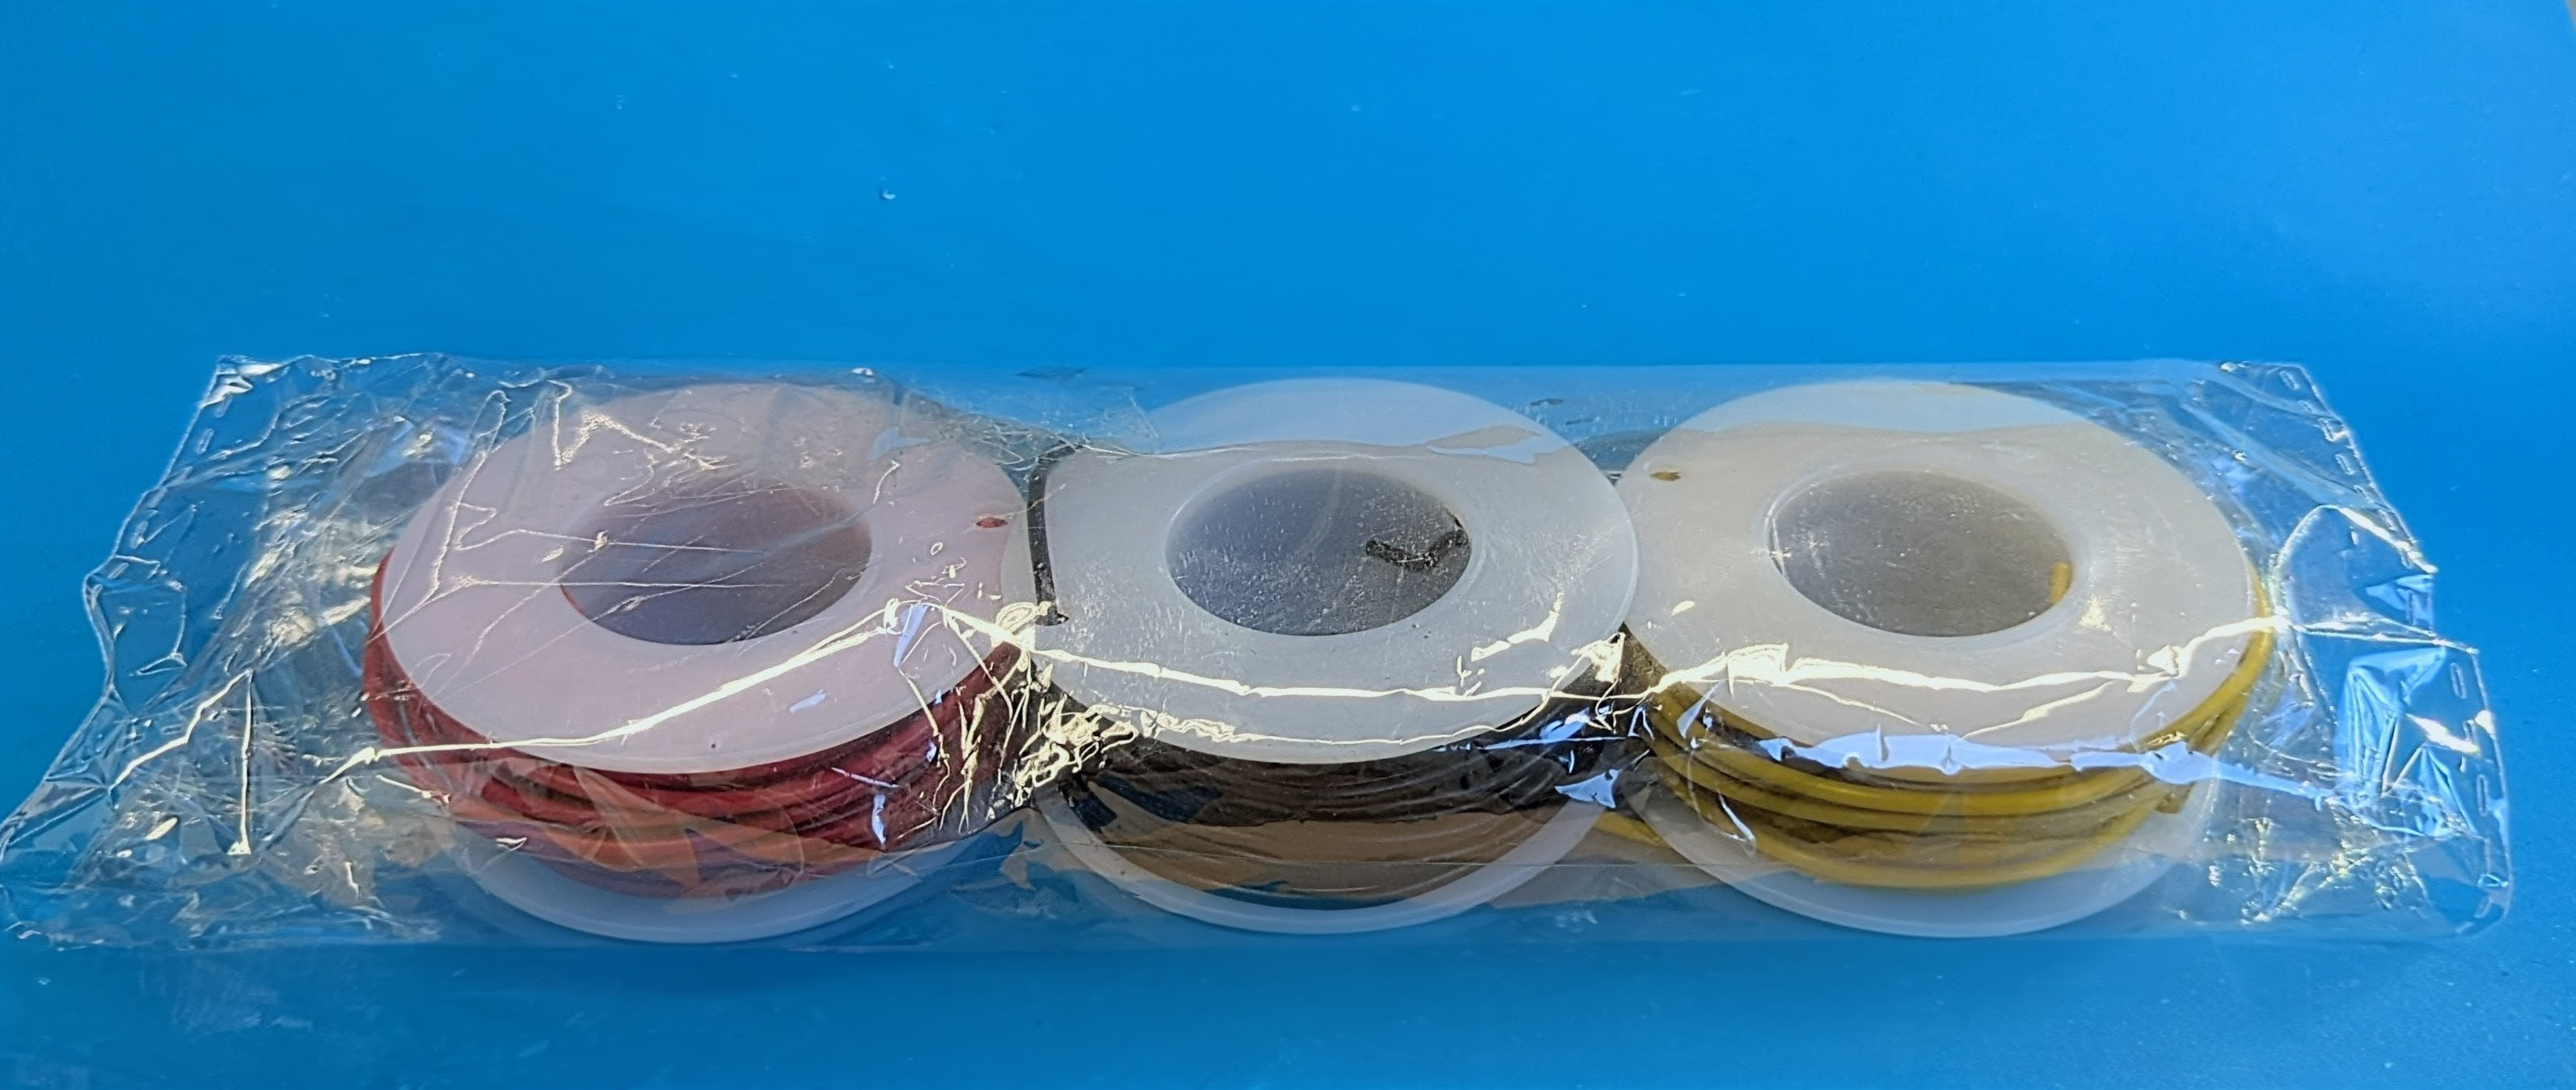
\includegraphics[width=\linewidth,keepaspectratio]{2.0.0.0_content/assets/bilder/projekt_kabel.jpg}
  \end{column}
\end{columns}
\end{frame}

\begin{frame}{Kabel fertig}
\begin{columns}[T]
  \begin{column}{0.58\textwidth}
    \small
    \begin{itemize}\setlength{\itemsep}{3mm}
      \item Sichtprüfung der Stecker
      \item Daten und Laden getestet
      \item Mitnahme möglich
    \end{itemize}
    \normalsize
  \end{column}
  \begin{column}{0.42\textwidth}
    \centering
    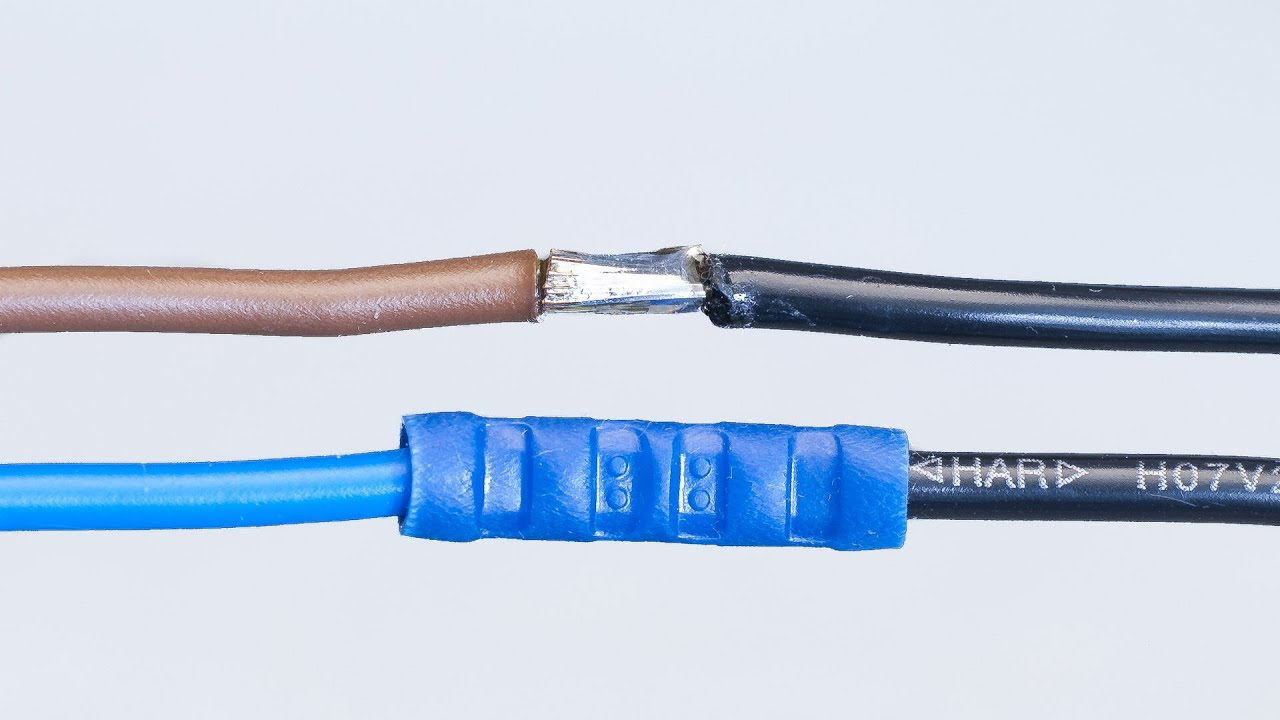
\includegraphics[width=\linewidth,keepaspectratio]{2.0.0.0_content/assets/bilder/projekt_kabel_fertig.jpg}
  \end{column}
\end{columns}
\end{frame}


\begin{frame}{Projektvorstellung kurz}
\begin{itemize}\setlength{\itemsep}{3mm}
  \item Was macht das Projekt
  \item Welche Teile werden gelötet
  \item Woran erkennst du Erfolg
\end{itemize}
\end{frame}

\begin{frame}{Sicherheit bei Projekten}
\begin{itemize}
  \item Richtige Temperatur wählen
  \item Bauteile nicht überhitzen
  \item Nach jedem Schritt prüfen
\end{itemize}
\end{frame}

\begin{frame}{Material und Rückgabe}
\begin{itemize}
  \item Teile pro Stufe ausgeben
  \item Reste sortiert sammeln
  \item Werkzeug ordentlich zurück
\end{itemize}
\end{frame}

\begin{frame}{Q \& A}
\begin{itemize}
  \item Fragen zum Pinecil
  \item Fragen zu Projekten
  \item Tipps für zu Hause
\end{itemize}
\end{frame}

\begin{frame}{Humor und Motivation}
\begin{itemize}
  \item Merke: Lötzinn, nicht Blödsinn
  \item Ziel: sicherer Start, kein Rekord
  \item Wir helfen dir gern
\end{itemize}
\end{frame}
